%%% New implementation section 

\section{Monitor Implementation}

%% paragraph 1 -- goals
To evaluate the feasibility of our monitoring algorithm for safety-critical real-time systems we have built a real-time CAN monitor on an ARM Cortex-M4 development board. This allowed us to explore the necessary optimizations and features required to perform real-time checking of realistic safety policies.

%% paragraph 2 -- what we built

%% Embedded restrictions
Software for safety-critical embedded systems typically contains more strict design constraints than less critical software. Two important and common constraints for these systems are avoiding recursion and not using dynamic memory allocations. 
% dynamic memory alloc
Common safety-critical coding guidelines discourage or prohibit dynamic memory allocation to avoid memory leaks.
Because our specification language is bounded, we can avoid dynamic allocation in our \monitor implementation by statically allocating space for the maximum number of entries for our history structures and other temporary data structures.
% recursion
Recursion is also usually prohibited because it can be difficult to guarantee a maximum stack depth when using recursion. Although \monitor utilizes recursion extensively, we can implement \monitor using a traditional iterative traversal of the specification formulas instead.

\subsection{Hybrid Algorithm}
Our eager monitoring algorithm attempts to evaluate specification rules as soon as possible, but this requires checking trace properties which may not be evaluated given the current trace. These unevaluated checks require extra computation time, and in general the majority of the policy evaluations performed by \monitor will be these eager checks which may not fully evaluate.

While early detection of violations can be useful, there are situations where eagerly checking an entire target specification may require more computation than is available from the monitor in a given period.

%
To enable the benefits of eager checking while avoiding the risks of losing real-time correctness, we have implemented a hybrid eager monitoring algorithm which performs non-eager (conservative) checking first and uses any spare time to eagerly check the remaining monitor residues.
%
Conservative \monitor monitoring is performed by only checking residues which are older than their formula delay, which guarantees that these residue will be reduced at their first evaluation.
%
Under our periodic sampling design, each step of conservative monitor only requires updating the history structures and checking a single residue (the oldest remaining one) for each specification policy.
%
This conservative check can be done quickly at each period, leaving any extra time until the next check for eager checking. This provides a conservative monitoring guarantee (\ie, the specification is checked within a known promptness delay) while also allowing the monitor to eagerly check as much of the specification as possible.

%As long as we know that the worst case execution time for message handing, incrementing the structures, and a single residue check is short enough to finish within a monitor period then we are guaranteed at least a conservatively correct and prompt output.

We have implemented the hybrid monitoring algorithm in our embedded monitor. The monitor updates the history structures (shared between the conservative and eager checking) and performs a conservative check once every monitoring period. It then uses the idle time between periods to perform eager checking of any remaining unchecked specification properties.
%
Figure \ref{fig:arch:oscope} shows the execution of the embedded monitor instrumented to output the currently executing task to an oscilloscope. 
This task output was captured using the specification used in the case study (see Section \ref{sec:case_study} plus another 200 time-step \emph{eventually} rule which was never satisfied. 
This means that at every step the monitor performed all 200 eager checks and could not reduce any remaining formulas. 
Even with this excess computation there was still a large portion of extra idle time -- 23ms of the 25ms loop was spent idle. 
This shows the eager checking finished reasonably quickly and the monitor could handle much longer formula durations or more complex formulas before the execution time becomes bad enough to require the hybrid algorithm for correctness guarantees. 

\begin{figure}
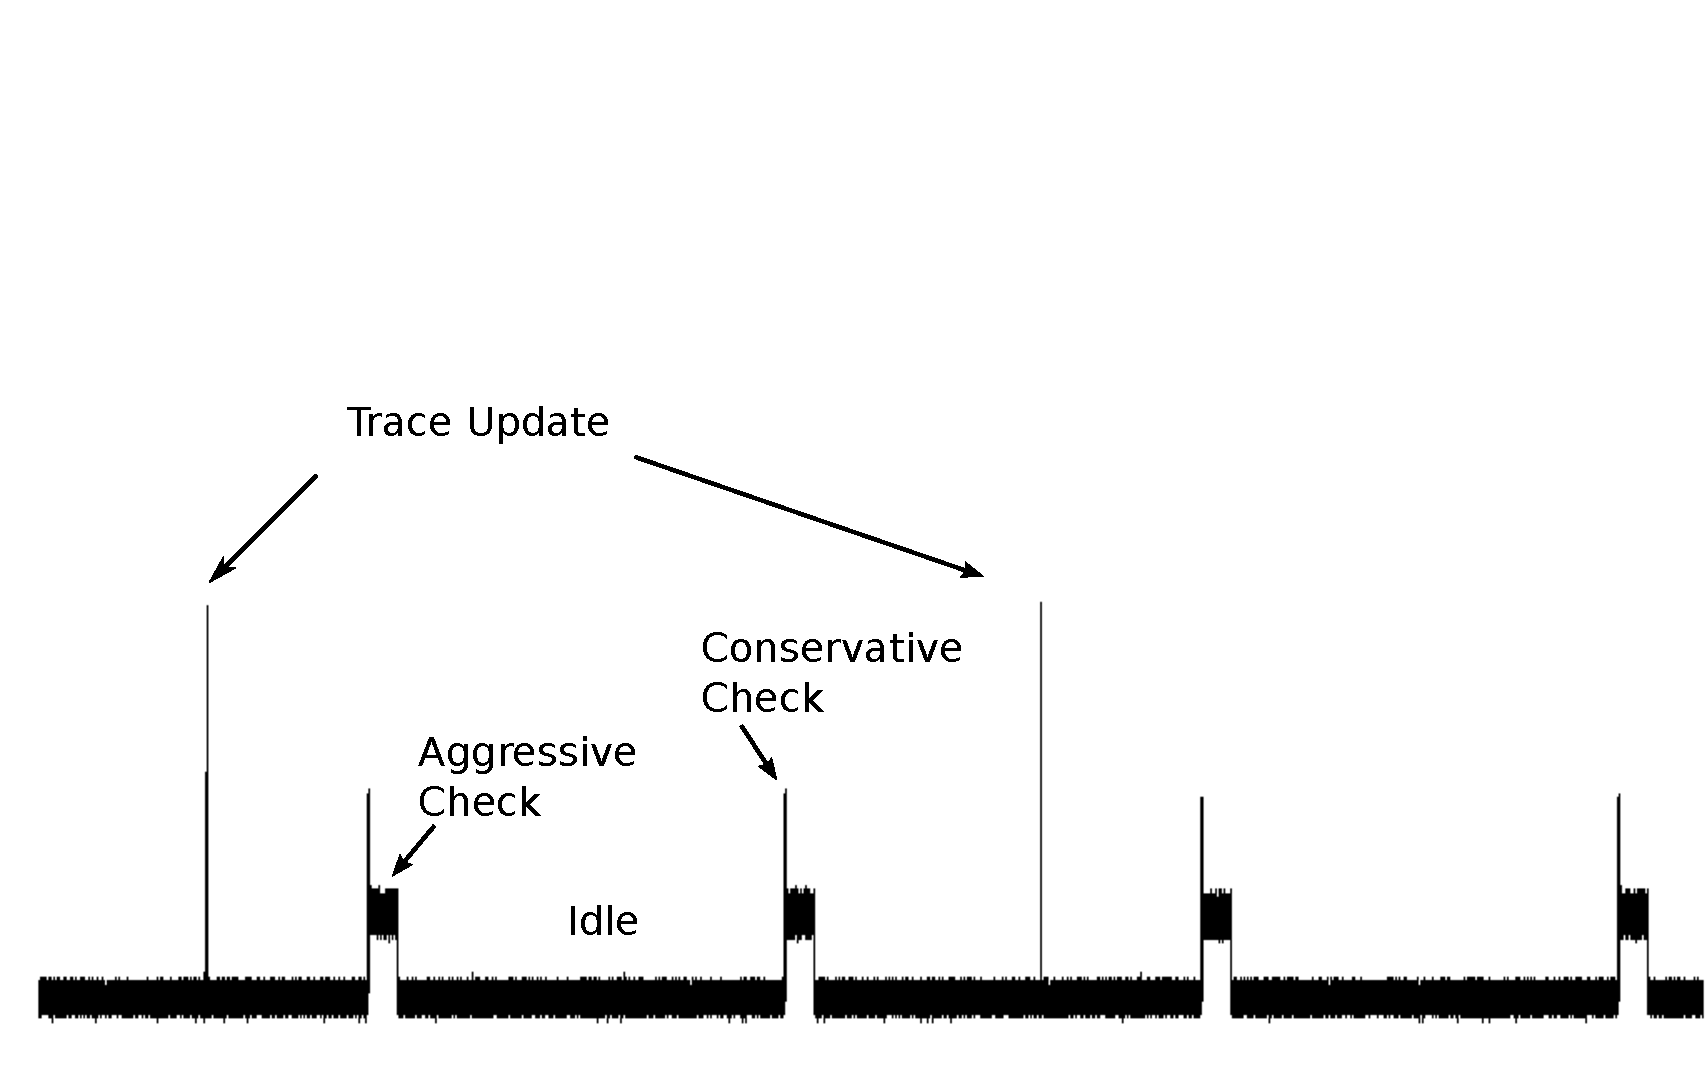
\includegraphics[width=4in]{img/scope_annotated}
\caption{Oscilloscope capture of embedded monitor task execution \label{fig:arch:oscope}}
\end{figure}
